\documentclass{article}
\usepackage[utf8]{inputenc}
\usepackage{amsmath}
\usepackage{graphicx}
\usepackage{tikz}
\usepackage{amssymb}
\usepackage{listings} % for the source code
\usepackage{xcolor} % for the source code as well
\DeclareUnicodeCharacter{2212}{\textendash}

% basic options for putting the source code
\definecolor{codegreen}{rgb}{0,0.6,0} 
\definecolor{codegray}{rgb}{0.5,0.5,0.5} \definecolor{codepurple}{rgb}{0.58,0,0.82} \definecolor{backcolour}{rgb}{0.95,0.95,0.92} 
\lstdefinestyle{mystyle}{ 
    backgroundcolor=\color{backcolour}, 
    commentstyle=\color{codegreen}, 
    keywordstyle=\color{magenta}, 
    numberstyle=\tiny\color{codegray}, 
    stringstyle=\color{codepurple}, 
    basicstyle=\ttfamily\footnotesize, 
    breakatwhitespace=false, 
    breaklines=true, 
    captionpos=b, 
    keepspaces=true, 
    numbers=left, 
    numbersep=5pt, 
    showspaces=false, 
    showstringspaces=false, 
    showtabs=false, 
    tabsize=2 } 
\lstset{style=mystyle}

\title{STAT387 HOMEWORK\#3 \linebreak \linebreak
\large INTRODUCTION TO STATISTICAL LEARNING}
\author{Saeah Go}
\date{Due February 22, 11:59 PM}

\begin{document}

\maketitle

\section*{{\underline{Conceptual}}}
\subsection*{1. 3(a, b; page 220)}
We now review $k$-fold cross-validation. \\
(a) Explain how $k$-fold cross-validation is implemented. \\
\indent The \textit{k-fold cross-validation} is implemented by randomly dividing the set of observations into $k$ groups, or folds, of approximately equal size. The first fold is treated in a validation set (test set), and the method is fit on the remaining $k-1$ folds. The mean squared error, $MSE_1$ is computed on the observations in the held-out fold. The procedure is repeated $k$ times. Each time, a different group of observations is treated as a validation set. This process results in k estimates of the test error, $MSE_1, MSE_2, \cdots, MSE_k$. And we compute the average of these errors. \\
(b) What are the advantages and disadvantages of $k$-fold cross-validation relative to: \\
\indent\indent i. The validation set approach? \\
\indent\indent\indent Advantages of k-fold cross validation: The validation set approach's estimate of the \textbf{test error rate can be highly variable}, depending on precisely which observations are included in the training set and which observations are included in the validation set. Also, validation set error rate may \textbf{tend to overestimate} the test error rate for the model fit on the entire data set, since it only uses half of the sample to fit the model (in general, a larger sample size leads to lower test error). \\
\indent\indent\indent Disadvantages of k-fold cross validation: Compare to the k-fold cross validation, the validation set approach is conceptually \textbf{simple and easy to implement}. Also, it takes \textbf{less computation} since it only fits the model once.

\indent\indent ii. LOOCV? \\
\indent\indent\indent Advantages of k-fold cross validation: LOOCV requires fitting the statistical learning method $n$ times. This means, it is possible that this method \textbf{could be computationally expensive} than k-fold cross validation. Also, k-fold cross validation often gives more accurate estimates of the test error rate than does LOOCV. \\ % lower variance and more accurate estimates 
\indent\indent\indent Disadvantages of k-fold cross validation: LOOCV has \textbf{less bias} than k-fold cross validation since it uses almost all of the points of the data set, nearly unbiased.

\section*{\underline{Applied}}
\subsection*{2. 13 (a, b, c, d, e, f, g, h, i; page 193)}
This question should be answered using the Weekly data set, which is part of the ISLR2 package. This data is similar in nature to the Smarket data from this chapter’s lab, except that it contains 1,089 weekly returns for 21 years, from the beginning of 1990 to the end of 2010. \\
(a) Produce some numerical and graphical summaries of the Weekly data. Do there appear to be any patterns? \\
\begin{center}
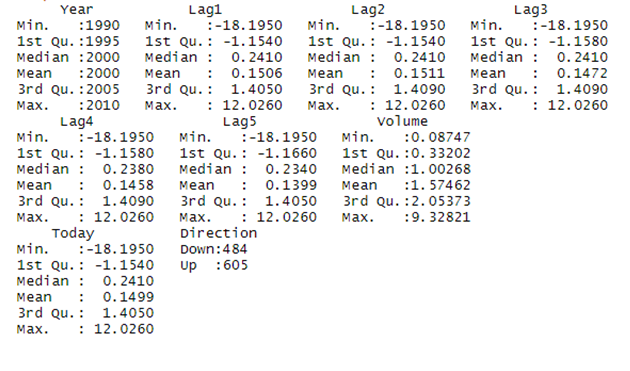
\includegraphics[scale = 0.46]{2.13.a - 1.png} \\
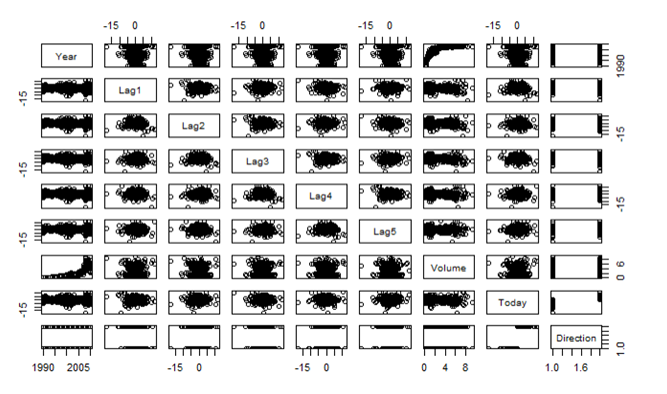
\includegraphics[scale = 0.46]{2.13.a - 2.png} \\
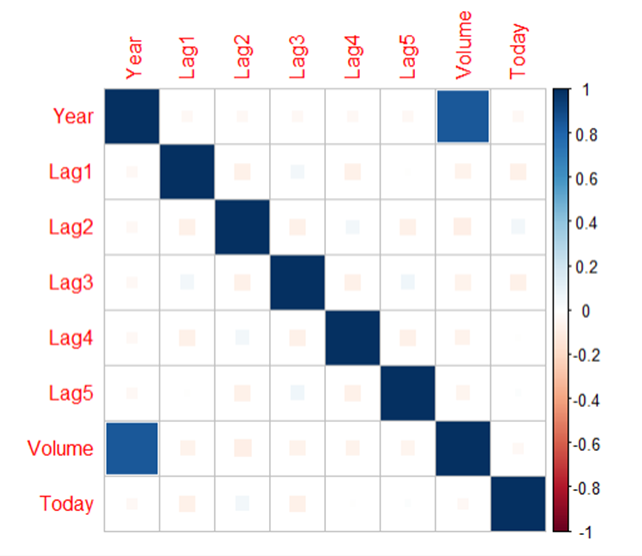
\includegraphics[scale = 0.46]{2.13.a - 3.png} \\
\end{center}
Through the third summary of data, the variables that appear to have any significant linear relation are Year and Volume. The correlation plot does not illustrate that any other variables are linearly related.\\
\linebreak (b) Use the full data set to perform a logistic regression with Direction as the response and the five lag variables plus Volume as predictors. Use the summary function to print the results. Do any of the predictors appear to be statistically significant? If so, which ones? \\
\begin{center}
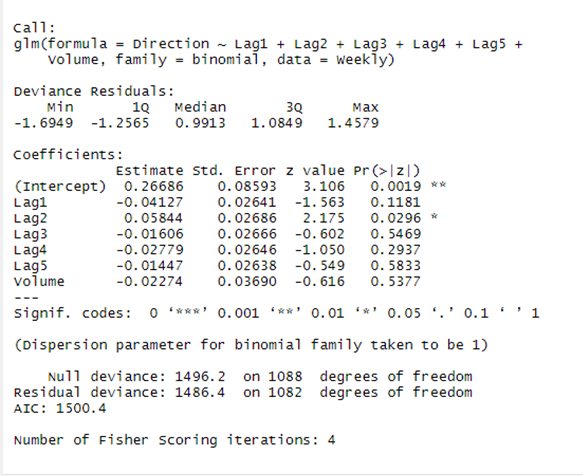
\includegraphics[scale = 0.46]{2.13.b.png} \\
\end{center}
$Lag2$ is the only variable that was statistically significant at the level of significance $\alpha = 0.05$. The other variables' p-values are all greater than $0.05$. \\%, which means those variables fail to reject the null hypothesis($\beta = 0$). \\
\linebreak (c) Compute the confusion matrix and overall fraction of correct predictions. Explain what the confusion matrix is telling you about the types of mistakes made by logistic regression. \\
The confusion matrix is: 
\begin{center}
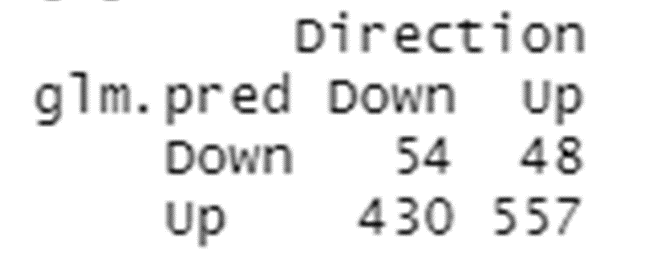
\includegraphics[scale = 0.46]{2.13.c.png} \\
\end{center}
The overall fraction of correct predictions is: 
\begin{center}
$\frac{TN + TP}{TN + FP + FN + TP} = \frac{54 + 557}{54 + 48 + 430 + 557} = \frac{611}{1089} = 0.5611 \approx 56.11\% $ \\
\end{center}
This illustrates that the model predicted the weekly market trend correctly $56.11\%$. \\
To talk about the types of mistakes made by logistic regression, there are false positive rate and false negative rate. The false positives are the cases that have been predicted as positive but they do not have that disease. And the false positive rate can be calculated as:
\begin{center}
$\frac{the \; number \; of \; negative \; events \; wrongly \; categorized \; as \; positive \; (false \; positives)}{the \; total \; number \; of actual \; negative \; events \; (regardless \; of \; classification)}$.

    $false positive = \frac{430}{54+430} = 0.8884 \approx 88.84\%$
\end{center}
Now, false negatives are the cases that have been predicted as negative but they actually have that disease.
\begin{center}
$\frac{the \; number \; of \; positive \; events \; wrongly \; categorized \; as \; negative \; (false \; negatives)}{the \; total \; number \; of actual \; positive \; events \; (regardless \; of \; classification)}$.

    $false positive = \frac{48}{48+557} = 0.9207 \approx 92.07\%$
\end{center}
(d) Now fit the logistic regression model using a training data period from 1990 to 2008, with $Lag2$ as the only predictor. Compute the confusion matrix and the overall fraction of correct predictions for the held out data (that is, the data from 2009 and 2010). \\
The confusion matrix is: 
\begin{center}
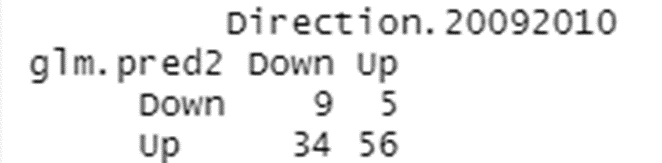
\includegraphics[scale = 0.46]{2.13.d.png} \\
\end{center}
The overall fraction of correct predictions for the held out data is: $(9 + 56)/(9 + 5 + 34 + 56) = 65/104 = 0.6250$. This means, when we split up the whole Weekly dataset into a training and test dataset, the model correctly predicted weekly trends at rate of 62.5\%, which is an improvement from the model that used the whole dataset. \\
\linebreak (e) Repeat (d) using LDA. \\
The confusion matrix is: 
\begin{center}
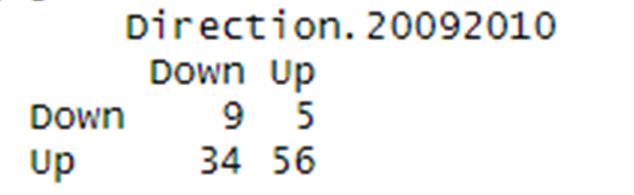
\includegraphics[scale = 0.46]{2.13.e.png} \\
\end{center}
The overall fraction of correct predictions for the held out data is: $(9 + 56)/(9 + 5 + 34 + 56) = 65/104 = 0.6250$. \\
\linebreak (f) Repeat (d) using QDA. \\
The confusion matrix is: 
\begin{center}
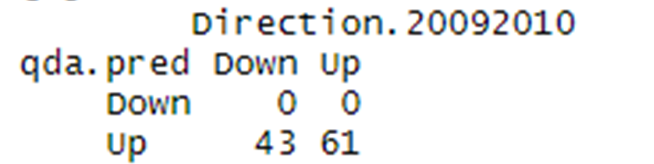
\includegraphics[scale = 0.46]{2.13.f.png} \\
\end{center}
The overall fraction of correct predictions for the held out data is: $(0 + 61)/(0 + 0 + 43 + 61) = 61/104 = 0.5865$. \\
\linebreak (g) Repeat (d) using KNN with $K = 1$. \\
The confusion matrix is: 
\begin{center}
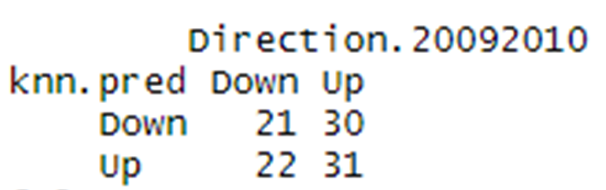
\includegraphics[scale = 0.46]{2.13.g.png} \\
\end{center}
The overall fraction of correct predictions for the held out data is: $(21 + 31)/(21 + 30 + 22 + 31) = 52/104 = 0.5$. \\
\linebreak (h) Repeat (d) using naive Bayes. \\
The confusion matrix is: 
\begin{center}
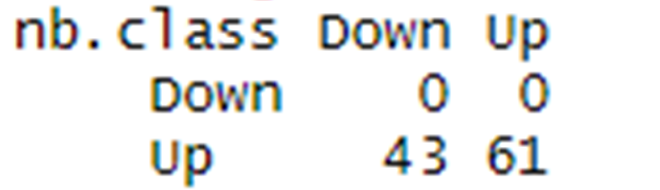
\includegraphics[scale = 0.46]{2.13.h.png} \\
\end{center}
The overall fraction of correct predictions for the held out data is: $(0 + 61)/(0 + 0 + 43 + 61) = 61/104 = 0.5865$. \\
\linebreak (i) Which of these methods appears to provide the best results on
this data? \\
\indent The methods that appear to provide the best results on this data are the Logistic Regression and Linear Discriminant Analysis. These both are having rates of $0.6250 = 62.5\%$.

\subsection*{3. 8 (a, b, c; pages 222-223)}
We will now perform cross-validation on a simulated data set. \\
(a) Generate a simulated data set as follows: 
\begin{lstlisting}[language=R]
> set.seed (1)
> x <- rnorm (100)
> y <- x - 2 * x ^2 + rnorm (100)
\end{lstlisting}
In this data set, what is $n$ and what is $p$? Write out the model used to generate the data in equation form. \\
\indent $n$ is $100$ and $p$ is $2$ ($x$ and $x^2$) since the model equation is $Y = X - 2X^2 + \epsilon$.
\linebreak (b) Create a scatterplot of $X$ against $Y$. Comment on what you find. \\
\begin{center}
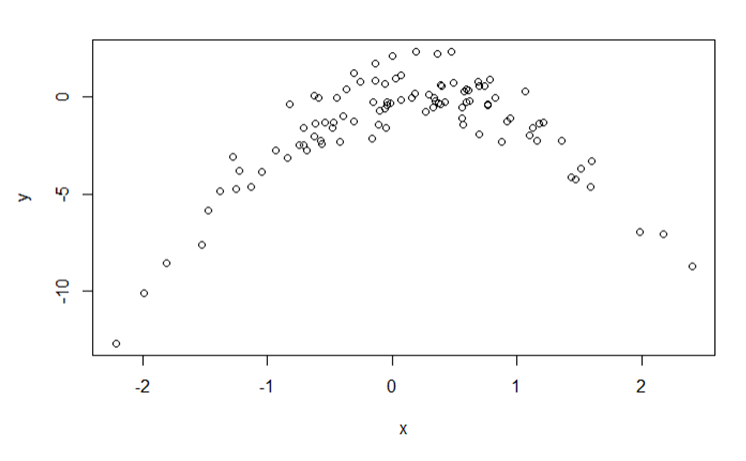
\includegraphics[scale = 0.46]{3.8.b.png} \\
\end{center}
I could see that the data shows us a curved relationship. \\
\linebreak (c) Set a random seed, and then compute the $LOOCV$ errors that result from fitting the following four models using least squares: \\
% is the error interval or just two errors
i. $Y = \beta_0 + \beta_1X + \epsilon$ \\
\indent The computed \textit{LOOCV} error for \textit{i} is: 7.288162 \\
\linebreak ii. $Y = \beta_0 + \beta_1X + \beta_2X^2 + \epsilon$ \\
\indent The computed \textit{LOOCV} error for \textit{ii} is: 0.9374236 \\
\linebreak iii. $Y = \beta_0 + \beta_1X + \beta_2X^2 + \beta_3X^3 + \epsilon$ \\
\indent The computed \textit{LOOCV} error for \textit{iii} is: 0.9566218 \\
\linebreak iv. $Y = \beta_0 + \beta_1X + \beta_2X^2 + \beta_3X^3 + \beta_4X^4 + \epsilon$ \\
\indent The computed \textit{LOOCV} error for \textit{iv} is: 0.9539049 \\
\linebreak Note you may find it helpful to use the data.frame() function to create a single data set containing both $X$ and $Y$.

\section*{\underline{R Code}}
\begin{lstlisting}[language=R]
# Applied

####################################
## 2.13 (a, b, c, d, e, f, g, h, i)
####################################
### Problem (a)
library(corrplot)
attach(Weekly)
summary(Weekly)
plot(Weekly)
corrplot(cor(Weekly[, -9]), method = "square")



### Problem (b)
glm.fit = glm(Direction ~ Lag1 + Lag2 + Lag3 + Lag4 + Lag5 + Volume, data = Weekly, family = binomial)
summary(glm.fit)



### Problem (c)
glm.probs <- predict(glm.fit, type = "response")
glm.pred <- rep("Down", 1089)
glm.pred[glm.probs > .5] <- "Up"

# create a confusion matrix
table(glm.pred, Direction)



### Problem (d)
train = (Year < 2009)
test = Weekly[!train,]
glm.fit2 = glm(Direction ~ Lag2, data = Weekly, family = binomial, subset = train)

# compute the confusion matrix
glm.probs2 <- predict(glm.fit2, test, type = "response")
glm.pred2 <- rep("Down", 104) # 104 is the length of glm.probs2
glm.pred2[glm.probs2 > .5] <- "Up"
Direction.20092010 = Direction[!train]
table(glm.pred2, Direction.20092010)

mean(glm.pred2 == Direction.20092010)



### Problem (e)
library(MASS)
lda.fit <- lda(Direction ~ Lag2, data = Weekly, family = binomial, subset = train)
lda.pred <- predict(lda.fit, test)
table(lda.pred$class, Direction.20092010)

mean(lda.pred == Direction.20092010)



### Problem (f)
qda.fit <- qda(Direction ~ Lag2, data = Weekly, subset = train)
qda.pred <- predict(qda.fit, test)$class
table(qda.pred, Direction.20092010)

mean(qda.pred == Direction.20092010)



### Problem (g)
library(class)
Weekly.train = as.matrix(Lag2[train])
Weekly.test = as.matrix(Lag2[!train])
train.Direction = Direction[train]
set.seed(1)
knn.pred = knn(Weekly.train, Weekly.test, train.Direction, k = 1)
table(knn.pred, Direction.20092010)

mean(knn.pred == Direction.20092010)



### Problem (h)
library(e1071)
nb.fit = naiveBayes(Direction ~ Lag2, data = Weekly, subset = train)
nb.class = predict(nb.fit, Direction.20092010)
table(nb.class, Direction.20092010)

mean(nb.class == Direction.20092010)









####################################
## 3.8 (a, b, c)
####################################
### Problem (a)
set.seed(1)
x <- rnorm(100) # vector
y <- x - 2 * x^2 + rnorm(100)



### Problem (b)
plot(x, y)



### Problem (c)
# i
library(boot) # need this library for LOOCV
Data = data.frame(x,y)
glm.fit1 = glm(y ~ x)
cv.err = cv.glm(Data, glm.fit1)
cv.err$delta

# ii
glm.fit2 = glm(y~poly(x,2))
cv.err = cv.glm(Data, glm.fit2)$delta[1]

# iii
glm.fit3 = glm(y~poly(x,3))
cv.err = cv.glm(Data, glm.fit3)$delta[1]

# iv
glm.fit4 = glm(y~poly(x,4))
cv.err = cv.glm(Data, glm.fit4)$delta[1]

cv.error <- rep(0,4)
for (i in 1:4) {
  glm.fit <- glm(y ~ poly(x, i), data = Data)
  cv.error[i] <- cv.glm(Data, glm.fit)$delta[1]
}
cv.error
\end{lstlisting}

\end{document}
